\chapter{Анализ проблематики}
\label{chapter1}

Программные ошибки могут иметь серьезные последствия, поэтому, при 
проектировнии программ с повышенными требованиями надежности используют 
формальную верификацию --- формальное доказательство соответствия предмета 
верификации его формальному описанию. Предметом здесь, например, могут являться 
алгоритмы, цифровые схемы.

Формальная верификация является трудозатратным процессом, который не всегда 
оправдан. Для упрощения данного процесса используются  различные системы 
автоматических доказательств. Под верификацией в данном случае понимается 
доказательство того что программа соответствует формальному описанию и что в 
программе отсутствуют ошибки \cite{certified}.

Существует ряд средств которые широко используются для автоматического 
доказательства теорем и автоматической верификации программ: ACL2, Coq, 
Isabelle/HOL, Twelf, PVS.

Система Coq является программным комплексом, предназначенный для
формализации и проверки правильности математических рассуждений.
Она представляет собой логическую среду, позволяющую описывать ма-
тематические теории и в интерактивном полуавтоматическом режиме
строить доказательства (формальные выводы). В основе системы ле-
жат интуиционистская логика и теория типов CIC (Calculus of Inductive
Constructions), что позволяет строить конструктивные доказательства и
извлекать из них соответствующие алгоритмы в виде верифицирован-
ных программ (поддерживаются языки функционального программиро-
вания OCaml, Haskell и Scheme). При этом правильность построенных
доказательств проверяется автоматически посредством сведения к зада-
че проверки правильности типизации термов в системе CIC\cite{msu}.


\section{Формальные основы системы Coq}
Coq --- интерактивное средство доказательства теорем, использующее свой 
функциональный язык Gallina с зависимыми типами. Формальной основой Coq 
является исчисление индуктивных конструкций (CIC), которое, в свою очередь, является расширение 
исчисления конструкций (CoC). Исчисление конструкций --- типизированное лямбда
-исчисление высшего порядка, разработанное Терри Коквандом.


\subsection{Исчисление конструкций}
Исчислений конструкций (CoC) находится на вершине лямбда-куба --- наглядной классификации типизированных лямбда-
исчислений с явным приписыванием типов. Куб организован в соответствии с 
возможными зависимостями между типами и термами этого исчисления\cite{pirs}.

\begin{figure}[ht]
	\centering
		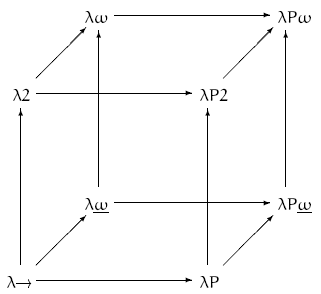
\includegraphics{img/Lambda_cube.png}
	\caption{Лямбда-куб}
	\label{fig:Lambda_cube}
\end{figure}

Базовой вершиной куба служит система $\lambda ^{\rightarrow }$ , 
соответствующая просто типизированному лямбда-исчислению. Термы (элементы 
сорта  $\ast$) зависят от термов; типы (элементы сорта $\Box$) в зависимостях 
не участвуют. 

Три оси, выходящие из базовой вершины, порождают следующие системы:
\begin{itemize}
	\item термы, зависящие от типов: система $\lambda 2$ (лямбда-исчисление с 
полиморфными типами, система F);
	\item типы, зависящие от типов: система $\lambda {\underline {\omega }}$ (
лямбда-исчисление с операторами над типами);
	\item типы, зависящие от термов: система $\lambda P$ (лямбда-исчисление с 
зависимыми типами).
\end{itemize}

Остальные системы представляют собой различные комбинации перечисленных 
зависимостей. Система $\lambda P\omega$  (полиморфное $\lambda$-исчисление 
высшего порядка с зависимыми типами)  фактически представляет собой 
исчисление конструкций. Далее рассмотрим подробнее системы $\lambda 2$, $
\lambda {\underline {\omega }}$ и $\lambda P$ которые в совокупности 
представляют собой чистое исчисление конструкций.


\textbf{Полиморфные типы.}

Система F ---  полиморфное $\lambda$-исчисление ---  
система типизированного лямбда-исчисления, отличающаяся от просто 
типизированной системы наличием механизма универсальной квантификации над 
типами\cite{pirs}.

Системy F иногда так-же называют лямбда-исчислением второго порядка ($\lambda$
2), поскольку по соответствию Карри-Говарда она аналогична интуиционистской 
логике второго порядка, в которой разрешена квантификация не только по 
отдельным объектам (термам), но и по предикатам (типам)\cite{pirs}.

Определение Системы F является естественным расширением $\lambda_{\rightarrow
}$, простого типизированного лямбда-исчисления. В $\lambda_{\rightarrow}$ $
\lambda$-абстракция служит для абстрагирования типов из термов, а с помощью
применения вместо абстрагированных частей подставляются значения.

Мотивацией для подобного рода расширения простого типизированного $\lambda$-
исчисления послужила следующая ситуация --- определенное поведение применимо 
к аргументам различного типа, например, удваивающая функция, которая может 
быть применена к типу Nat, Bool, Fun и другим. Такия ситуация в простом 
типизированом $\lambda$-исчислении решается с помощью написания функции для 
каждого типа. Наличие нескольких функций, каждая из которых применима к 
своему типу аргумента (типы аргуметов различны 
для разных функций), но эти функции ведут себя одинаково нарушает один 
из принципов разработки программ - принцип абстракции\cite{pirs}: каждая 
существенная область функциональности в программе должна быть реализована 
всего в одном месте программного кода. Если различные фрагменты кода 
реализуют аналогичную функциональность, то, как правило, имеет
смысл слить их в один фрагмент, абстрагируя различающиеся части.

Таким образом,  нужен способ абстрагировать тип терма, а затем 
конкретизировать абстрактный терм аннотациями нужного типа. Для 
абстрагирования типов из термов, а также для последующего заполнения 
абстракций вводится новая форма абстракции $\lambda X.t$, параметром который 
служит тип, и новую форму применения, $t \ [T]$, в которой аргументом служит 
выражение типа\cite{girard}. 

Синтаксис полиморфного $\lambda$-исчисления:

Термы: $t \ ::= \ x \ | \ \lambda x: T.t \ | \ t \ t \ | \ \lambda X.t \ | \ t \ [T]$

Значения: $v \ ::= \ \lambda X:T.t \ | \lambda X.t$

Типы: $T \ ::= \ X \ | \ T \rightarrow T \ | \ \forall X.T$

Контексты: $\Gamma \ ::= \ \emptyset \ | \ \Gamma , \ x:T \ | \Gamma , X$

Вычисление:

\begin{mathpar}
	\inferrule{
		t_{1} \ \rightarrow \ t_{2}
	} {
		t_{1} \: t \ \rightarrow \ t_{2} \: t
	} \and 
	\inferrule{
		t_{1} \ \rightarrow \ t_{2}
	} {
		v \: t_{1} \ \rightarrow \ v \: t_{2}
	} \and 
	\inferrule{
		( \lambda x:T_{11}.t_{12}) \: v \ \rightarrow \ [ x\mapsto v] t_{12}
	}{	} \and 
	\inferrule{
		t_{1} \ \rightarrow \ t_{2}
	}{
		t_{1} \: [T] \ \rightarrow \ t_{2} \: [T]
	} \and 
	\inferrule{
		\lambda X.t \: [T] \ \rightarrow \ [X \mapsto T] \: t
	}{	} 
\end{mathpar}

Типизация: 

\begin{mathpar}
	\inferrule{
		x:T \: \in \: \Gamma
	} {
		\Gamma \: \vdash \: x:T
	} \and 
	\inferrule{
		\Gamma , \ x:T_{1} \ \vdash \ t_{2}:T_{2}
	} {
		\Gamma \ \vdash \ \lambda x:T_{1}.t_{2} \: : \: T_{1} \rightarrow T_{2}
	} \and 
	\inferrule{
		\Gamma \ \vdash \ t_{1}:T_{11}\rightarrow T_{12} \\ \Gamma \ \vdash \ t_{2}:T_{11}
	}{
			\Gamma \ \vdash \ t_{1} \: t_{2} \: : \: T_{12}
		} \and 
	\inferrule{
		\Gamma , \ X \ \vdash \ t: T
	}{
		\Gamma \ \vdash \lambda X.t \: : \: \forall X.T
	} \and 
	\inferrule{
		\Gamma \ \vdash t \: : \: \forall X.T
	}{	
		\Gamma \ \vdash t [T_{1}] \ : \ [X \: \rightarrow T_{1}] T
	} 
\end{mathpar}


\textbf {Система $\lambda{\underline {\omega }}$}
Пирс 465 операции над типами 

\textbf{Зависимые типы}

Зависимые типы, впервые, были использованы в различных системах, направленных 
на построение и проверку автоматических доказательств. С практической точки 
зрения, зависимый тип --- тип, который зависит от значения объекта. В 
качестве простейшего примера можно рассмотреть тип $String_{n}$ --- бинарные 
строки длинны $n$. Данный тип записит от выбора n, который имеет 
тип натурального числа (n: int). Согласно изоморфизму Карри-Говарда  оператор 
создания такого типа из натурального числа соответствует предикат по int. 
Такой предикат называют конструктором типа\cite{lectures}.

Классификация конструкторов в соответствие с их доменоми вводит понятие сорта (
kind): конструктор $String_{n}$ имеет сорт $int \Rightarrow *$, где $*$ --- сорт всех типов.

Определение объекта типа $String_{n}$ может оказаться однородным по $n$, то 
есть может существовать общая процедура, которая ведет себя обинаково со 
строками любой длинны, например, превращает их в строку из нулей длинны $n$. 
Типом такой процедуры является $(\forall x: \ int) \ String_{x}$\cite{lectures, ml}.

В общем случае, тип вида $(\forall x: \ T) \ \sigma$ является типом функции, 
применимой к объектам типа $T$ и возвращающий объект типа $\sigma \ [x:=a]$ 
для каждого аргумента $a: \ T$. Эта идея является более общей, чем идея типа 
функции ($\rightarrow$), если $x$ не является свободной переменной в $\sigma$, то тип $(\forall x: \ T) \ \sigma$ является типом $T \rightarrow \sigma$ \cite{lectures, hofmanndt}.

Теоретико-множественным аналогом зависимого типа является продукция (
произведение). Если $\{A_{t}\} \ t \in T$ является индексированым семейством 
множеств, то продукция этого семейства множество:
\begin{figure}[ht]
	\centering
		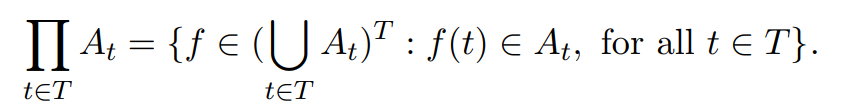
\includegraphics[width=0.70\textwidth]{img/set.png}
	\label{fig:set}
\end{figure}

Для $f \in \Pi_{t \in T} A _{t}$ значение $f(t)$ принадлежат множеству $A _{
t}$, предположительно рахличном для каждого значения агрумента. Если все $A _{
t}$ равны фиксированному множеству $A$, то получится равенство: $\Pi_{t \in 
T} A_{t} = A ^{T}$, что еще раз подтверждает соотношение $\rightarrow$ с $
\forall$.Таким образом, импликация является частным случаем квантором всеобщности.

Как в случае и с другими теориям типов, системы с зависимыми типами 
базируются на теоретическом $\lambda$-исчислении с абстрактным синтаксисом, 
правилами типизациии и оценки \cite{ml, hofmanndt}. $\lambda$-исчисление с 
зависимыми типами является системой $\lambda P$. Система $\lambda P$
является большим расширением простого типизированного $\lambda$-исчисления, 
даже без введения квантора существования. Рассмотрим данную систему не вводя 
квантор существования\cite{lectures}.

Имеются три сорта выражений: объекты-выражения, конструкторы и сорта. Тип 
рассматривается как частный случай конструктора. Контексты в системе $\lambda 
P$ определяются как последовательность предположений, не всякая 
последовательность объявлений может рассматриваться как валидный контекст, 
зависит от выводимости определенных суждений. 

Вводится константа для сорта --- $\ast$.

Синтаксис $\lambda P$ \cite{lectures, advanced}:

Термы: $t \ ::= \ x \ \  | \ \  \lambda x:T.t \ \ | \ t \ t$

Типы: $T \ ::= \ X \ \ | \ \  \Pi x:T.T \ \  | \ \  T \ t $

Сорта: $K \ ::= \ \ast \ \ | \  \Pi x:T.K$

Контексты: $\Gamma \ ::= \ \oslash \ \  | \  \ \Gamma , \ x:T \ \ | \ \ \Gamma , \ X::K$

Валидные сорта:

\begin{figure}[ht]
  \centering
    \begin{mathpar}
      \inferrule{
        \Gamma \vdash \ast
      } {} \and 
      \inferrule{
       \Gamma \ \vdash \  T:: \ast \\ \Gamma , \  x:T \ \vdash K
      }{
        \Gamma \ \vdash \Pi{x: \ T.K}
      } 
    \end{mathpar}
\end{figure}

Правила приписывания сорта:
\begin{figure}[ht]
  \centering
    \begin{mathpar}
      \inferrule{
        \Gamma \  \vdash \ T\ ::\ \ast \\ \Gamma , \ \vdash \ K
      } {\Gamma \ \vdash \ x::K} \and 
      \inferrule{
       \Gamma \ \vdash \  T_{1}:: \ast \\ \Gamma , \  x:T_{1} \ \vdash T_{2}:: \ast
      }{
        \Gamma \ \vdash \Pi x: \ T_{1}.T_{2} :: \ast
      } \and
      \inferrule{
       \Gamma \ \vdash \  S:: \Pi x: \ T.K \\ \Gamma  \ \vdash t :: T
      }{
        \Gamma \ S t : [x \mapsto t] K
      } \and 
      \inferrule{
       \Gamma \ \vdash \  T :: K \\ \Gamma \ \vdash K \equiv K^{`}
      }{
        \Gamma \ \vdash \ T :: K^{`}
      } 
    \end{mathpar}
\end{figure}


Правила типизации:
\begin{figure}[ht]
  \centering
    \begin{mathpar}
      \inferrule{
        x:T \ \in \Gamma \  \\ \Gamma \ \vdash \ T :: \ast
      } {\Gamma \ \vdash \ x:T} \and 
      \inferrule{
       \Gamma \ \vdash \  S :: \ast \\ \Gamma , \  x:S \ \vdash t : T
      }{
        \Gamma \ \vdash \  \lambda x:S.t \  : \ \Pi x: \ S.T
      } \and
      \inferrule{
       \Gamma \ \vdash \  t_{1}:: \Pi x: \ S.T \\ \Gamma  \ \vdash t_{2} :: S
      }{
        \Gamma \ t_{1} \ t_{2} : [x \mapsto t_{2}] T
      } \and 
      \inferrule{
       \Gamma \ \vdash \  t : T \\ \Gamma \ \vdash T \equiv T^{`} :: \ast
      }{
        \Gamma \ \vdash \ t : T^{`}
      } 
    \end{mathpar}
\end{figure}

В приведенных выше правилах типизации и приписывания сорта используется 
понятие эквивалентности сорта и типа. Правила, согласно которым два сорта или 
типа можно считать эквивалентными приведены в приложении.

Согласно изоморфизму Карри-Говарда зависимым типам соответсвует логика 
предикатов первого порядка\cite{lectures, hofmanndt}. Предикат B над типом А рассматривается как 
функция значения типа над A, и, следовательно, универсальное квантификация 
совпадает с зависимым продуктом: $\forall \ x: \  A.B (x)$ эквивалентно $\Pi \ x: \ A.B(x)$


Зависимые типы позволяют перенести некоторые вычисления на фазу проверки 
типов, предостовляя при этом возможность создавать более выразительные 
доказательства используя изоморфизм Карри-Говарда.



\textbf{Исчисление конструкций}

Наиболее развитой в $\lambda$-кубе системой является --- это $\lambda P _{
\omega}$, также известная как исчисление конструкций (Calculus of 
Constructions). 
Основное преимущество чистого исчисления конструкций --- <<замкнутость системы
>>,где математические и вычислительные нотации могут быть представлены с 
использованием квантификации высшего порядка\cite{pauline}. Однако это 
представление является не удовлетворительным как с вычислительной, так и 
с логической точек зрения. Это привело к расширению данной теории индуктивными 
определениями как объектами первого класса \cite{coq, pfenning}, которое 
называется исчисление индуктивных конструкций (Calculus of Inductive 
Constructions).
В качестве индуктивного определения можно рассмотреть пример следующего 
определения натураьных чисел: натуральное число $n$ --- это либо $z$ (zero, 
ноль), либо $S \ m$ (следующее за натуральным числом $m$).

Исчисление конструкций расширяет $\lambda$-исчисление с зависимыми типами 
следующим образом\cite{advanced}: вводится новый валидный терм: $all \ x:T.t$
; вводятся типы Prop --- утверждения (propositions) и Prf --- семейство 
доказательств. Элементы типа Prop представляют собой утверждения и типы 
данных (не типы доказальства утвержений), напрмер, натуральные числа. 
Семейство типов Prf присваивает каждому утверждению или типу данных
$p \ : \ Prop$ тип $Prf \ p$ этого доказательства или в случае типов данных 
его членов.
Вводятся следующие правила приписывания сорта и типизации:
\begin{itemize}
	\item приписывание сорта:
    \begin{mathpar}
      \inferrule{
        \Gamma \ \vdash \ Prop \ :: \ \ast
      } {} \and 
      \inferrule{
       \Gamma \ \vdash \  Prf \ :: \ \Pi x: Prop.\ast
      }{} 
    \end{mathpar}
		
		\item типизация:
		
		\begin{mathpar}
      \inferrule{
        \Gamma \ \vdash \ T \ :: \ \ast \\ \Gamma , \ x:T \ \vdash \ t:Prop
      } {
				\Gamma \ \vdash \ all \ x:T.t \ : \ Prop
			} 
    \end{mathpar}
\end{itemize}


\subsection{Индуктивные типы}


